\documentclass{../vespers-booklet}
\usepackage{multicol}

\begin{document}

% TODO: Update the title for the specific feast
\chapter*{Second Vespers of the Most Precious Blood of Our Lord Jesus Christ}

\vspace{0.5cm}

\begin{center}
	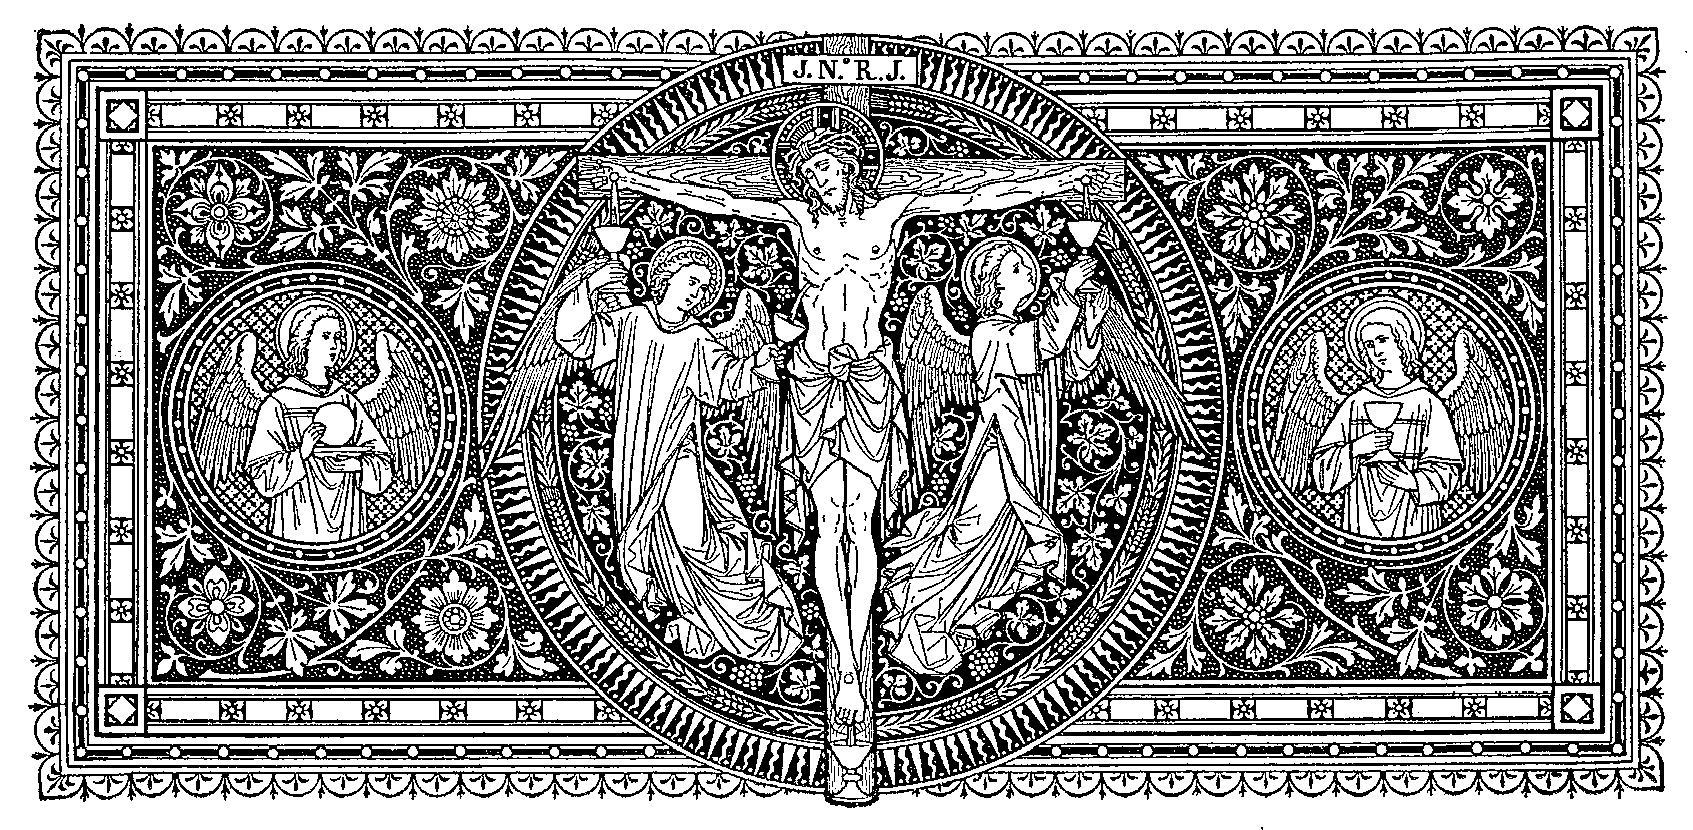
\includegraphics[width=\textwidth]{crucifix-and-Eucharist.jpg}
\end{center}

\vfill\pagebreak

%\section*{Beginning of the Office}

\begin{rubricbox}

{\color{red}When the Officiant kneels, all \textbf{kneel} and pray silently one \textit{Pater noster} (Our Father) and \textit{Ave Maria} (Hail Mary). Then all rise with the Officiant make the sign of the cross with him as he intones:}

\end{rubricbox}

% TODO: Make sure that the tone of the deus adjutorium matches the season primarily and the solemnity of the feast secondarily
 \gresetinitiallines{1}
\gregorioscore{../common/deus-in-adjutorium-solemn}

\textit{
O God, come to my assistance.
{\color{red}\Rbar.}~O Lord, make haste to help me.
Glory be to the Father, and to the Son, and to the Holy Spirit,
as it was in the beginning, is now, and ever shall be, world without end. Amen.
Praise to Thee, O Lord, King of endless glory.}

\vfill\pagebreak

%TODO: Add that the correct psalms, and verify that their tones, and their associated pointed text are correct

\section*{Psalm 109}

\textit{\textnormal{Ant. 1.} Who is this that * cometh from Edom, with dyed garments from Bozrah? this, that is glorious in His apparel?
 \textnormal{Ps.} The Lord said to my Lord: * Sit thou at my right hand.}
 
 \begin{rubricbox}

{\color{red}All remain standing throughout the first antiphon.
After the psalm is intoned by the Cantor, all \textbf{sit} at the asterisk.}

\end{rubricbox}

\gresetinitiallines{1}
\gregorioscore{ps109-antiphon}

\gresetinitiallines{0}
\gregorioscore{ps109-intonation}

 \begin{latinenglishsection}

\latinenglish{

	2. Donec ponam ini\textbf{mí}cos \textbf{tu}os,~* scabéllum \textbf{pe}dum tu\textbf{ó}rum.

3. Virgam virtútis tuæ emíttet Dómi\textbf{nus} ex \textbf{Si}on:~* domináre in médio inimi\textbf{có}rum tu\textbf{ó}rum.

4. Tecum princípium in die virtútis tuæ in splendóri\textbf{bus} sanc\textbf{tó}rum:~* ex útero ante lucíferum \textbf{gé}nu\textbf{i} te.

5. Jurávit Dóminus, et non poeni\textbf{té}bit \textbf{e}um:~* Tu es sacérdos in ætérnum secúndum órdi\textbf{nem} Mel\textbf{chí}sedech.

6. Dóminus a \textbf{dex}tris \textbf{tu}is,~* confrégit in die iræ \textbf{su}æ \textbf{re}ges.

7. Judicábit in natiónibus, im\textbf{plé}bit ru\textbf{í}nas:~* conquassábit cápita in \textbf{ter}ra mul\textbf{tó}rum.

8. De torrénte in \textbf{vi}a \textbf{bi}bet:~* {\color{red}\textit{(stand)}} proptérea exal\textbf{tá}bit \textbf{ca}put.

{\color{red}\textit{(bow)}} Glória \textbf{Pa}tri, et \textbf{Fí}lio,~* et Spi\textbf{rí}tui \textbf{Sanc}to.

{\color{red}\textit{(rise)}} Sicut erat in princípio, et \textbf{nunc}, et \textbf{sem}per,~* et in s\'{\ae}cula sæcu\textbf{ló}rum. \textbf{A}men. %%

}{
	% 1. The Lord said to my Lord: Sit thou at my right hand:

2. Until I make thy enemies thy footstool.
 
3. The Lord will send forth the sceptre of thy power out of Sion: rule thou in the midst of thy enemies.
 
4. With thee is the principality in the day of thy strength: in the brightness of the saints:
 from the womb before the day star I begot thee.
 
5. The Lord hath sworn, and he will not repent: Thou art a priest for ever according to the order of Melchisedech.
 
6. The Lord at thy right hand hath broken kings in the day of his wrath.

7. He shall judge among nations, he shall fill ruins: he shall crush the heads in the land of the many.

8. He shall drink of the torrent in the way: therefore shall he lift up the head. 

Glory be. %%
}

\end{latinenglishsection}

\gresetinitiallines{1}
\gregorioscore{ps109-antiphon}

\section*{Psalm 110}

\textit{\textnormal{Ant. 2.} I that speak * in righteousness, mighty to save.
 \textnormal{Ps.} I will praise thee, O Lord, with my whole heart; * in the council of the just, and in the congregation.}
 
 \begin{rubricbox}

{\color{red}The remaining Psalms are said in the same manner as the first.}

\end{rubricbox}

\gresetinitiallines{1}
\gregorioscore{ps110-antiphon}

\gresetinitiallines{0}
\gregorioscore{ps110-intonation}

 \begin{latinenglishsection}

\latinenglish{

	2. Magna \textbf{ó}pera \textbf{Dó}mini:~* exquisíta in omnes volun\textbf{tá}tes \textbf{e}jus.

3. Conféssio et magnificéntia \textbf{o}pus \textbf{e}jus:~* et justítia ejus manet in \textbf{s\'{\ae}}culum \textbf{s\'{\ae}}culi.

4. Memóriam fecit mirabílium suórum,~{\color{red}\GreDagger}\ miséricors et mise\textbf{rá}tor \textbf{Dó}minus:~* escam dedit ti\textbf{mén}ti\textbf{bus} se.

5. Memor erit in s\'{\ae}culum testa\textbf{mén}ti \textbf{su}i:~* virtútem óperum suórum annuntiábit \textbf{pó}pulo \textbf{su}o:

6. Ut det illis heredi\textbf{tá}tem \textbf{gén}tium:~* ópera mánuum ejus véritas, \textbf{et}\\ ju\textbf{dí}cium.

7. Fidélia ómnia mandáta ejus:~{\color{red}\GreDagger}\ confirmáta in \textbf{s\'{\ae}}culum \textbf{s\'{\ae}}culi,~* facta in veritáte et \textbf{æ}qui\textbf{tá}te.

8. Redemptiónem misit \textbf{pó}pulo \textbf{su}o:~* mandávit in ætérnum\\ testa\textbf{mén}tum \textbf{su}um.

9. Sanctum, et terríbile \textbf{no}men \textbf{e}jus:~* inítium sapiéntiæ \textbf{ti}mor \textbf{Dó}mini.

10. Intelléctus bonus ómnibus faci\textbf{én}tibus \textbf{e}um:~* laudátio ejus manet in \textbf{s\'{\ae}}culum \textbf{s\'{\ae}}culi.

\textit{(bow)} Glória \textbf{Pa}tri, et \textbf{Fí}lio,~* et Spi\textbf{rí}tui \textbf{Sanc}to.

\textit{(rise)} Sicut erat in princípio, et \textbf{nunc}, et \textbf{sem}per,~* et in s\'{\ae}cula sæcu\textbf{ló}rum. \textbf{A}men. %%

}{
	 1. I will praise thee, O Lord, with my whole heart; in the council of the just: and in the congregation.
 
 2. Great are the works of the Lord: sought out according to all his wills.
 
 3. His work is praise and magnificence: and his justice continueth for ever and ever.
 
 4.  He hath made a remembrance of his wonderful works, being a merciful and gracious Lord: he hath given food to them that fear him. 	
 
 5. He will be mindful for ever of his covenant: he will shew forth to his people the power of his works.
 
 6. That he may give them the inheritance of the Gentiles: the works of his hands are truth and judgment.
 
 7. All his commandments are faithful: confirmed for ever and ever, made in truth and equity.
 
 8. He hath sent redemption to his people: he hath commanded his covenant for ever.
 
 9. Holy and terrible is his name: the fear of the Lord is the beginning of wisdom.
 
 10. A good understanding to all that do it: his praise continueth for ever and ever.  %%
}

\end{latinenglishsection}

\vfill\pagebreak

\gresetinitiallines{1}
\gregorioscore{ps110-antiphon}

\section*{Psalm 111}

\textit{\textnormal{Ant. 3.} He was clothed * with a vesture dipped in blood, and His name is called The Word of God.
 \textnormal{Ps.} Blessed is the man that feareth the Lord: * he shall delight exceedingly in his commandments.}

\gresetinitiallines{1}
\gregorioscore{ps111-antiphon}

\gresetinitiallines{0}
\gregorioscore{ps111-intonation}

 \begin{latinenglishsection}

\latinenglish{

	2. Potens in terra erit \textit{se}\textit{men} \textbf{e}jus:~* generátio rectórum \textit{be}\textit{ne}\textit{di}\textbf{cé}tur.

3. Glória, et divítiæ in \textit{do}\textit{mo} \textbf{e}jus:~* et justítia ejus manet in \textit{s\'{\ae}}\textit{cu}\textit{lum} \textbf{s\'{\ae}}culi.

4. Exórtum est in ténebris \textit{lu}\textit{men} \textbf{rec}tis:~* miséricors, et mise\textit{rá}\textit{tor}, \textit{et} \textbf{jus}tus.

5. Jucúndus homo qui miserétur et cómmodat,~\GreDagger\ dispónet sermónes suos \textit{in} \textit{ju}\textbf{dí}cio:~* quia in ætérnum \textit{non} \textit{com}\textit{mo}\textbf{vé}bitur.

6. In memória ætérna \textit{e}\textit{rit} \textbf{jus}tus:~* ab auditióne ma\textit{la} \textit{non} \textit{ti}\textbf{mé}bit.

7. Parátum cor ejus speráre in Dómino,~\GreDagger\ confirmátum \textit{est} \textit{cor} \textbf{e}jus:~* non commovébitur donec despíciat in\textit{i}\textit{mí}\textit{cos} \textbf{su}os.

8. Dispérsit, dedit paupéribus:~\GreDagger\ justítia ejus manet in s\'{\ae}\textit{cu}\textit{lum} \textbf{s\'{\ae}}culi,~* cornu ejus exaltá\textit{bi}\textit{tur} \textit{in} \textbf{gló}ria.

9. Peccátor vidébit, et irascétur,~\GreDagger\ déntibus suis fremet \textit{et} \textit{ta}\textbf{bé}scet:~* {\color{red}\textit{(stand)}} desidérium pecca\textit{tó}\textit{rum} \textit{per}\textbf{í}bit.

{\color{red}\textit{(bow)}} Glória Pa\textit{tri}, \textit{et} \textbf{Fí}lio,~* et Spi\textit{rí}\textit{tu}\textit{i} \textbf{Sanc}to.

{\color{red}\textit{(rise)}} Sicut erat in princípio, et \textit{nunc}, \textit{et} \textbf{sem}per,~* et in s\'{\ae}cula sæ\textit{cu}\textit{ló}\textit{rum}. \textbf{A}men. %%

}{
	1. Blessed is the man that feareth the Lord: he shall delight exceedingly in his commandments.

2. His seed shall be mighty upon earth: the generation of the righteous shall be blessed.

3. Glory and wealth shall be in his house: and his justice remaineth for ever and ever.

4. To the righteous a light is risen up in darkness: he is merciful, and compassionate and just.

5. Acceptable is the man that sheweth mercy and lendeth: he shall order his words with judgment:
because he shall not be moved for ever.

6. The just shall be in everlasting remembrance: he shall not fear the evil hearing.

7. His heart is ready to hope in the Lord: his heart is strengthened, he shall not be moved until he look over his enemies.

8. He hath distributed, he hath given to the poor: his justice remaineth for ever and ever: his horn shall be exalted in glory.

9. The wicked shall see, and shall be angry, he shall gnash with his teeth and pine away: the desire of the wicked shall perish.  %%
}

\end{latinenglishsection}

\gresetinitiallines{1}
\gregorioscore{ps111-antiphon}

\vfill\pagebreak

\section*{Psalm 112}

\textit{\textnormal{Ant. 4.} Wherefore art Thou * red in thine apparel, and thy garments like him that treadeth in the wine-vat?
 \textnormal{Ps.} Praise the Lord, ye children: * praise ye the name of the Lord.}

\gresetinitiallines{1}
\gregorioscore{ps112-antiphon}

\gresetinitiallines{0}
\gregorioscore{ps112-intonation}

 \begin{latinenglishsection}

\latinenglish{

	2. \textit{(bow)} Sit nomen Dómini bene\textbf{díc}tum,~*
	ex hoc nunc, et us\textit{que} \textit{in} \textbf{s\'{\ae}}culum.

3. A solis ortu usque ad oc\textbf{cá}sum,~*
	laudábile \textit{no}\textit{men} \textbf{Dó}mini.

4. Excélsus super omnes gentes \textbf{Dó}minus,~*
	et super cælos gló\textit{ri}\textit{a} \textbf{e}jus.

5. Quis sicut Dóminus, Deus noster, qui in altis \textbf{há}bitat,~*
	et humília réspicit in cælo \textit{et} \textit{in} \textbf{ter}ra?

6. Súscitans a terra \textbf{ín}opem,~*
	et de stércore é\textit{ri}\textit{gens} \textbf{páu}perem:

7. Ut cóllocet eum cum prin\textbf{cí}pibus, *
	cum princípibus pó\textit{pu}\textit{li} \textbf{su}i.

8. Qui habitáre facit stérilem in \textbf{do}mo,~* {\color{red}\textit{(stand)}}
	matrem filió\textit{rum} \textit{læ}\textbf{tán}tem.

{\color{red}\textit{(bow)}} Glória Patri, et \textbf{Fí}lio,~*
	et Spirí\textit{tu}\textit{i} \textbf{Sanc}to.

{\color{red}\textit{(rise)}} Sicut erat in princípio, et nunc, et \textbf{sem}per,~*
	et in s\'{\ae}cula sæcu\textit{ló}\textit{rum}. \textbf{A}men. %%

}{
	%1. Praise the Lord, ye children: praise ye the name of the Lord.
 	
2. Blessed be the name of the Lord, from henceforth now and for ever.
 	
3. From the rising of the sun unto the going down of the same, the name of the Lord is worthy of praise.
 	
4. The Lord is high above all nations; and his glory above the heavens.
 	
5.Who is as the Lord our God, who dwelleth on high, and looketh down on the low things in heaven and in earth?
 	
6. Raising up the needy from the earth, and lifting up the poor out of the dunghill:
 	
7. That he may place him with princes, with the princes of his people.
 	
8. Who maketh a barren woman to dwell in a house, the joyful mother of children. 

Glory be. %%
}

\end{latinenglishsection}

\gresetinitiallines{1}
\gregorioscore{ps112-antiphon}

\section*{Psalm 147}

\textit{\textnormal{Ant. 5.} I have trodden * the wine-press alone, and of the people there was none with Me.
 \textnormal{Ps.} Praise the Lord, O Jerusalem: * praise thy God, O Sion.}

\gresetinitiallines{1}
\gregorioscore{ps147-antiphon}

\gresetinitiallines{0}
\gregorioscore{ps147-intonation}

 \begin{latinenglishsection}

\latinenglish{

	2. Quóniam confortávit seras\\ portárum tu\textbf{á}rum:~* benedíxit fíliis tu\textit{is} \textbf{in} te.

3. Qui pósuit fines tuos \textbf{pa}cem:~* et ádipe fruménti sá\textit{ti}\textbf{at} te.

4. Qui emíttit elóquium suum \textbf{ter}ræ:~* velóciter currit ser\textit{mo} \textbf{e}jus.

5. Qui dat nivem sicut \textbf{la}nam:~* nébulam sicut cíne\textit{rem} \textbf{spar}git.

6. Mittit crystállum suam sicut buc\textbf{cél}las:~* ante fáciem frígoris ejus quis sus\textit{ti}\textbf{né}bit?

7. Emíttet verbum suum, et\\ liquefáciet \textbf{e}a:~* flabit spíritus ejus, et flu\textit{ent} \textbf{a}quæ.

8. Qui annúntiat verbum suum \textbf{Ja}cob:~* justítias, et judícia su\textit{a} \textbf{Is}raël.

9. Non fecit táliter omni nati\textbf{ó}ni:~* {\color{red}\textit{(stand)}} et judícia sua non\\ manifestá\textit{vit} \textbf{e}is.

{\color{red}\textit{(bow)}} Glória Patri, et \textbf{Fí}lio,~* et Spirítu\textit{i} \textbf{Sanc}to.

{\color{red}\textit{(rise)}} Sicut erat in princípio, et nunc, et \textbf{sem}per,~* et in s\'{\ae}cula sæculó\textit{rum}. \textbf{A}men. %%

}{
	%1. Praise the Lord, O Jerusalem: praise thy God, O Sion.

2. Because he hath strengthened the bolts of thy gates, he hath blessed thy children within thee.

3. Who hath placed peace in thy borders: and filleth thee with the fat of corn.

4. Who sendeth forth his speech to the earth: his word runneth swiftly.

5. Who giveth snow like wool: scattereth mists like ashes.

6. He sendeth his crystal like morsels: who shall stand before the face of his cold?

7. He shall send out his word, and shall melt them: his wind shall blow, and the waters shall run.

8. Who declareth his word to Jacob: his justices and his judgments to Israel.

9. He hath not done in like manner to every nation: and his judgments he hath not made manifest to them.

Glory be. %%
}

\end{latinenglishsection}

\gresetinitiallines{1}
\gregorioscore{ps147-antiphon}

%\begin{rubricbox}

%{\color{red}The antiphon is repeated: \textit{Quis est iste\dots}} %%

%\end{rubricbox}

%TODO: Verify that the little chapter is fitting for the feast

\vfill\pagebreak

\section*{Little Chapter (Hebrews 9:11-12)}

\textit{\color{red}The Officiant leads the Little Chapter:}

\begin{latinenglishsection}

\latinenglish{
	Fratres: Christus assistens póntifex futurórum bonórum, per ámplius et perféctius tabernáculum non\\ manufáctum, id est, non hujus creatiónis: {\color{red}\GreDagger} neque per sánguinem hircórum, aut vitulórum, sed per próprium sánguinem introívit semel in Sancta, ætérna redemptióne\\ invénta. 
	{\color{red}\Rbar.}~Deo grátias.
}{
	Brethren, Christ being come, a high priest of the good things to come, by a greater and more perfect tabernacle, not made with hands, that is, not of this creation, neither by the blood of goats or of calves, but by His own blood, entered once into the Holies, having obtained eternal redemption. 
	 {\color{red}\Rbar.}~Thanks be to God.
}

\end{latinenglishsection}

\vfill\pagebreak

% TODO: Verify that the hymn is correct for the feast (including the responsory after the hymn)

\section*{Hymn}

\textit{\color{red}The Cantor leads the hymn:}

\gresetinitiallines{1}
\gregorioscore{../hymns/festivis_resonent}
% Translation from: https://tosingistopraytwice.wordpress.com/2017/03/29/forth-let-the-long-procession-stream/
{\itshape
	1.  Forth let the long procession stream,
	And through the streets in order wend;
	Let the bright waving line of torches gleam,
	The solemn chant ascend.
	
	2. While we, with tears and sighs profound,
	That memorable Blood record,
	Which, stretch’d on his hard Cross, from many a wound
	The dying Jesus pour’d.
	
	3. By the first Adam’s fatal sin
	Came death upon the human race;
	In this new Adam doth new life begin,
	And everlasting grace.
	
	4. For scarce the Father heard from Heaven
	The cry of his expiring Son,
	When in that cry our sins were all forgiven,
	And boundless pardon won.
	
	5. Henceforth, whoso in that dear Blood
	Washeth, shall lose his every stain;
	And in immortal roseate beauty rob’d,
	An angel’s likeness gain.
	
	6. Only, run thou with courage on
	Straight to the goal set in the skies;
	He, who assists thy course, will give thee soon
	The everlasting prize.
	
	7. Father supreme! vouchsafe that we,
	For whom thine only Son was slain,
	And whom thy Holy Ghost doth sanctify,
	May heavenly joys attain.
}

\textit{\color{red}The Cantor says the following before all reply afterwards:}

\gresetinitiallines{0}
\gabcsnippet{
(c3) <c><sp>V/</sp>.</c> Te(h) er(h)go(h), quáe(h)su(h)mus(h), tu(h)is(h) fá(h)mu(h)lis(h) súb(h)ve(h)ni.(g'_/hvGF'E/fgf.) (::)
}

\gresetinitiallines{0}
\gabcsnippet{
(c3) <c><sp>R/</sp>.</c> Quos(h) pre(h)ti(h)ó(h)so(h) sán(h)gui(h)ne(h) re(h)de(h)mís(h)ti.(g'_/hvGF'E/fgf.) (::)
}

\textit{{\color{red}\Vbar.}~We therefore pray Thee, help Thy servants.
{\color{red}\Rbar.}~O Thou hast redeemed us with Thy precious blood.}

\vfill\pagebreak

\section*{Magnificat}

\textit{\textnormal{Ant Magn.} Behold a faithful and prudent servant, whom the Lord has set over His household.
\textnormal{Cant.} My soul doth magnify the Lord: and my spirit hath rejoiced in God my Saviour.}

\begin{rubricbox}

{\color{red}The Cantor leads by intoning the antiphon and the first verse.}

\end{rubricbox}

\gresetinitiallines{1}
\gregorioscore{magnificat-antiphon-only}

\begin{rubricbox}

{\color{red}All \textbf{remain standing} and make the sign of the cross with the Cantor.}

\end{rubricbox}

\gresetinitiallines{0}
\gregorioscore{magnificat-intonation}

 \begin{latinenglishsection}

\latinenglish{	
3. Quia respéxit humilitátem \textit{an}\textit{cíl}\textit{læ} \textbf{su}æ:~* ecce enim ex hoc beátam me dicent omnes gene\textit{ra}\textit{ti}\textbf{ó}nes.

4. Quia fecit mihi \textit{ma}\textit{gna} \textit{qui} \textbf{pot}\textbf{ens} est:~* et sanctum \textit{no}\textit{men} \textbf{e}jus.

5. Et misericórdia ejus a progéni\textit{e} \textit{in} \textit{pro}\textbf{gé}\textbf{ni}es~* timén\textit{ti}\textit{bus} \textbf{e}um.

6. Fecit poténtiam in \textit{brá}\textit{chi}\textit{o} \textbf{su}o:~* dispérsit supérbos mente \textit{cor}\textit{dis} \textbf{su}i.

7. Depósuit pot\textit{én}\textit{tes} \textit{de} \textbf{se}de,~* et exal\textit{tá}\textit{vit} \textbf{hú}\textbf{mi}les.

8. Esuriéntes \textit{im}\textit{plé}\textit{vit} \textbf{bo}nis:~* et dívites dimí\textit{sit} \textit{in}\textbf{á}nes.

9. Suscépit Israël \textit{pú}\textit{e}\textit{rum} \textbf{su}um,~* recordátus misericór\textit{di}\textit{æ} \textbf{su}æ.

10. Sicut locútus est \textit{ad} \textit{pa}\textit{tres} \textbf{nos}tros,~* Abraham et sémini e\textit{jus} \textit{in} \textbf{s\'{\ae}}\textbf{cu}la.
}{	
	1. My soul doth magnify the Lord.

2. And my spirit hath rejoiced in God my Saviour.

3. Because he hath regarded the humility of his handmaid; for behold from henceforth all generations shall call me blessed.

4. Because he that is mighty, hath done great things to me; and holy is his name.

5. And his mercy is from generation unto generations, to them that fear him.

6. He hath shewed might in his arm: he hath scattered the proud in the conceit of their heart.

7. He hath put down the mighty from their seat, and hath exalted the humble.

8. He hath filled the hungry with good things; and the rich he hath sent empty away.

9. He hath received Israel his servant, being mindful of his mercy: 

10. As he spoke to our fathers, to Abraham and to his seed for ever. 
}

\end{latinenglishsection}

\textit{\color{red}(bow)} Glória Patri, et \textbf{Fí}lio,~* 
	et Spirí\textit{tu}\textit{i} \textbf{Sanc}to.

\textit{\color{red}(rise)} Sicut erat in princípio, et nunc, et \textbf{sem}per,~*
	et in s\'{\ae}cula sæcu\textit{ló}\textit{rum}. \textbf{A}men.

\gresetinitiallines{0}
\gregorioscore{magnificat-antiphon-only}

\begin{rubricbox}

{\color{red}All  \textbf{remain standing}.}

\end{rubricbox}

\vfill\pagebreak

\section*{Collect}

\textit{\color{red}The Officiant leads the collect:}

\begin{latinenglishsection}
% Concluding collect from the Litany of the Most Precious Blood: https://www.ewtn.com/catholicism/library/litany-of-the-most-precious-blood-of-our-lord-jesus-christ-11888
\latinenglish{
	{\color{red}\Vbar.}~Dómine exáudi oratiónem meam.\\
	{\color{red}\Rbar.}~Et clamor meus ad te véniat.
	
	Orémus.
	Omnipotens sempiterne Deus, qui unigenitum Filium tuum mundi Redemptorem constituisti, ac ejus sanguine placari voluisti: {\color{red}\GreDagger} concede, quaesumus, salutis nostrae pretium solemni cultu ita venerari, atque a praesentis vitae malis ejus virtute defendi in terris; * ut fructu perpetuo laetemur in caelis. Per eumdem Dominum nostrum Iesum Christum Filium Tuum, qui vivit et regnat in unitate Spiritu Sancti, Deus, per omnia saecula saeculurom.
	{\color{red}\Rbar.}~Amen.
}{
	{\color{red}\Vbar.}~Lord, hear my prayer.
	{\color{red}\Rbar.}~And let my cry come unto Thee.
	
	Let us pray.
	Almighty and eternal God, Thou hast appointed Thine only-begotten Son the Redeemer of the world and willed to be appeased by his blood. Grant, we beg of Thee, that we may worthily adore this price of our salvation and through its power be safeguarded from the evils of the present life so that we may rejoice in its fruits forever in heaven. Through the very same Jesus Christ Thy Son, who liveth and reigneth with Thee in the unity of the Holy Spirit, God, world without end.
	{\color{red}\Rbar.}~Amen.
}
\end{latinenglishsection}

%TODO: Add commemorations for the date

\textit{\color{red}For commemorations, the Cantor intones the antiphon and says the responsorial prayer afterwards. The Officiant prays the associated collect.}

\section*{Commemoration of the Visitation of the Blessed Virgin Mary}

\textit{\textnormal{Ant.} Blessed art thou, Mary, who didst believe the Lord; what the Lord said to thee shall be fulfilled in thee. Alleluia.}

\gresetinitiallines{1}
\gregorioscore{../commemorations/an--beata_es_maria--solesmes}

\begin{latinenglishsection}

\latinenglish{
	{\color{red}\Vbar.}~Benedicta tu in mulieribus.\\
	{\color{red}\Rbar.}~Et benedictus fructus ventris tui.
	
	Orémus.
	Famulis tuis, quaesumus Domine, caelestis gratiae munus impertire: {\color{red}\GreDagger} ut quibus beatae Virginis partus exstitit salutis ex6rdium, • Visitati6nis ejus votiva solemnitas pacis tribuat incre- mentum.
}{
	{\color{red}\Vbar.}~Blessed art thou amongst women.
	{\color{red}\Rbar.}~And blessed is the fruit of thy womb.
	
	Let us pray.
	Grant, O Lord, we beseech thee, unto all thy servants, the gift of thine heavenly grace, that even as the Blessed Virgin being made a Mother hath been unto them the first step unto their salvation, so the godly and solemn memorial of her Visitation may be the bringer of an increase of peace.
}

\end{latinenglishsection}

\section*{Commemoration of the Friday within the Octave of the Sacred Heart of Jesus}

\textit{\textnormal{Ant.}  But when they came to Jesus and saw that he was dead already, they broke not his legs, but one of the soldiers with a spear pierced his side, and forthwith came there out Blood and Water.}

\gresetinitiallines{1}
\gregorioscore{../commemorations/an--ad_jesum_autem--solesmes}

\begin{latinenglishsection}
\latinenglish{
	{\color{red}\Vbar.}~Hauriétis aquas in gáudio.\\
	{\color{red}\Rbar.}~De fóntibus Salvatóris.
	
	Orémus.
Deus, qui nobis in Corde Fílii tui, nostris vulneráto peccátis, infinítos dilectiónis thesáuros\\ misericórditer largíri dignáris;\\ concéde, qu\'{\ae}sumus, ut illi devótum pietátis nostræ præstántes\\ obséquium, dignæ quoque\\ satisfactiónis exhibeámus offícium.
	Per Dóminum nostrum Jesum\\ Christum Fílium tuum, qui tecum vivit et regnat in unitáte Spíritus Sancti, Deus, per ómnia s\'{\ae}cula sæculórum.
}{
	{\color{red}\Vbar.}~With joy shall ye draw water.
	{\color{red}\Rbar.}~Out of the fountains of the Saviour.
	
	Let us pray.
	O God, who hast suffered the Heart of thy Son to be wounded by our sins, and in that very Heart hast bestowed on us the abundant riches of thy love: grant that the devout homage of our hearts, which we render unto him, may of thy mercy be deemed a recompence acceptable in thy sight.
	Through Jesus Christ, thy Son, Our Lord, Who liveth and reigneth with thee in the unity of the Holy Ghost, God, world without end.
}
\end{latinenglishsection}

\textit{\color{red}The Officiant leads the following:}

\begin{latinenglishsection}

\latinenglish{
	{\color{red}\Vbar.} Dómine exáudi oratiónem meam.\\
	{\color{red}\Vbar.} Et clamor meus ad te véniat.
}{
	{\color{red}\Vbar.} Lord, hear my prayer. {\color{red}\Rbar.} And let my cry come unto Thee.
	{\color{red}\Vbar.} Let us bless the Lord. {\color{red}\Rbar.} Thanks be to God.
}

\end{latinenglishsection}

%\vfill\pagebreak

\textit{\color{red}The Cantor leads the Benedicamus:}

\gresetinitiallines{1}
\gregorioscore{../common/benedicamus-2v-solem}

\textit{\color{red}The Officiant leads the following:}

\begin{latinenglishsection}

\latinenglish{
	{\color{red}\Vbar.} Fidélium ánimæ, per\\ misericórdiam Dei, requiéscant in pace. \\
	{\color{red}\Rbar.} Amen.
}{
	{\color{red}\Vbar.} May the souls of the faithful departed, through the mercy of God, rest in peace. {\color{red}\Rbar.}~Amen.
}

\latinenglish{
	Pater noster \textit{(silently)}.
}{
	Our Father\dots
}

\latinenglish{
	{\color{red}\Vbar.} Dóminus det nobis suam pacem. \\
	{\color{red}\Rbar.} Et vitam ætérnam. Amen.
}{
	{\color{red}\Vbar.} May the Lord grant us his peace. 
	{\color{red}\Rbar.} And life eternal. Amen.
}

\end{latinenglishsection}

%TODO: Add the Marian Anthem for the season and verify that the oration afterwards is correct

\vfill\pagebreak

\section*{Marian Anthem}

\textit{\color{red}The Cantor leads the Marian anthem and responses afterwards; the Officiant leads the ending collect:}

\gresetinitiallines{1}
\gregorioscore{../marian-anthems/salve-regina-solemn-tone}

{\itshape
	Hail, holy Queen, Mother of mercy, our life, our sweetness and our hope.
	To thee do we cry, poor banished children of Eve. 
	To thee do we send up our sighs, mourning and weeping in this valley of tears. 
	Turn, then, most gracious advocate, thine eyes of mercy toward us, 
	and after this, our exile, show unto us the blessed fruit of thy womb, Jesus. 
	O clement, O loving, O sweet Virgin Mary.
}

\begin{latinenglishsection}

\latinenglish{
	{\color{red}\Vbar.} Ora pro nobis, sancta Dei Genitrix.\\
	{\color{red}\Rbar.} Ut digni efficamur promissionibus Christi.
	
	Oremus. 
	Omnipotens sempiterne Deus, qui gloriosae Virginis Matris Mariae corpus et animam, ut dignum Filii tui habitaculum effici mereretur, Spiritu Sancto cooperante\\ praeparasti, da, ut cuius\\ commemoratione laetamur; eius pia intercessione, ab instantibus malis et a morte perpetua liberemur. Per eundem Christum Dominum\\ nostrum.
	{\color{red}\Rbar.} Amen.
}{
	{\color{red}\Vbar.} Pray for us, O holy Mother of God.
	{\color{red}\Rbar.} That we may be made worthy of the promises of Christ.
	
	Let us pray. 
	Almighty and everlasting God, Who by the working of the Holy Spirit didst prepare both body and soul of the glorious Virgin Mother, Mary, that she might deserve to be made a worthy dwelling for Thy Son, grant that we who rejoice in her memory, may, by her loving intercession, be delivered from present evils and from lasting death, through the same Christ our Lord. 
	{\color{red}\Rbar.} Amen.
}
\end{latinenglishsection}

\textit{\color{red}The Officiant leads the following:}

\begin{latinenglishsection}

\latinenglish{
	{\color{red}\Vbar.} Divínum auxílium máneat semper nobíscum.\\
	{\color{red}\Rbar.} Amen.
}{
	May the divine assistance remain always with us.\\
	{\color{red}\Rbar.}~Amen.
}
\end{latinenglishsection}

\begin{rubricbox}

{\color{red} After the Office, all \textbf{kneel} and pray in silence for a time.}

\end{rubricbox}

\end{document}